\documentclass[11pt,letterpaper]{article}
\usepackage[utf8]{inputenc}

%----- Configuración del estilo del documento------%
\usepackage{epsfig,graphicx}
\usepackage[left=2cm,right=2cm,top=1.8cm,bottom=2.3cm]{geometry}
\usepackage{fancyhdr}
\usepackage{lastpage}
\usepackage{url}
\pagestyle{fancy}
\fancyhf{}
\rfoot{\textit{Página \thepage \hspace{1pt} de \pageref{LastPage}}}


%------ Paquetes matemáticos básicos --------%
\usepackage{amsmath}
\usepackage{amssymb}
\usepackage{amsthm}

\usepackage[spanish]{babel}
\usepackage{graphicx}
\usepackage{hyperref}

\usepackage{tabularx}
\usepackage{xcolor}
\usepackage[table]{xcolor}
\usepackage{colortbl}
\usepackage{array, multirow, multicol, tabularx}
\usepackage{tcolorbox}
\newtheorem{theorem}{Theorem}[section]
\newtheorem{corollary}{Corollary}[theorem]
\newtheorem{lemma}[theorem]{Lemma}

%------si-------%
\definecolor{B}{HTML}{FFFFFF}
\definecolor{G}{HTML}{5e5e5e}
\definecolor{R2}{HTML}{d53d40}
\definecolor{A2}{HTML}{034190}
\definecolor{V2}{HTML}{7faa50}
\newcommand{\R}{\mathbb{R}}
\newcommand{\C}{\mathcal{C}}
\newcommand{\N}{\mathbb{N}}
\newcommand{\Z}{\mathbb{Z}}
\newcommand{\Q}{\mathbb{Q}}
\renewcommand{\theenumi}{\Roman{enumi}}
\renewcommand{\labelenumi}{{\theenumi}.}

\begin{document}

%------ Encabezado -------- %

\begin{center}
    \begin{minipage}{3cm}
    	\begin{center}
    		\includegraphics[height=3.4cm]{logo_unam.png}
    	\end{center}
    \end{minipage}\hfill
    \begin{minipage}{10cm}
    	\begin{center}
    	\textbf{\large Universidad Nacional Autónoma de México}\\[0.1cm]
        \textbf{Facultad de Ciencias}\\[0.1cm]
        \textbf{\'Algebra superior 1}\\[0.1cm]
        ¿El $0$ es natural?\\[0.1cm]
         El\'ias L\'opez Rivera\\[0.1cm]
        \texttt{ elias.lopezr\,@ciencias.unam.mx }\\[0.1cm]
        Fecha:\,\,27/10/2024
    	\end{center}
    \end{minipage}\hfill
    \begin{minipage}{3cm}
    	\begin{center}
    		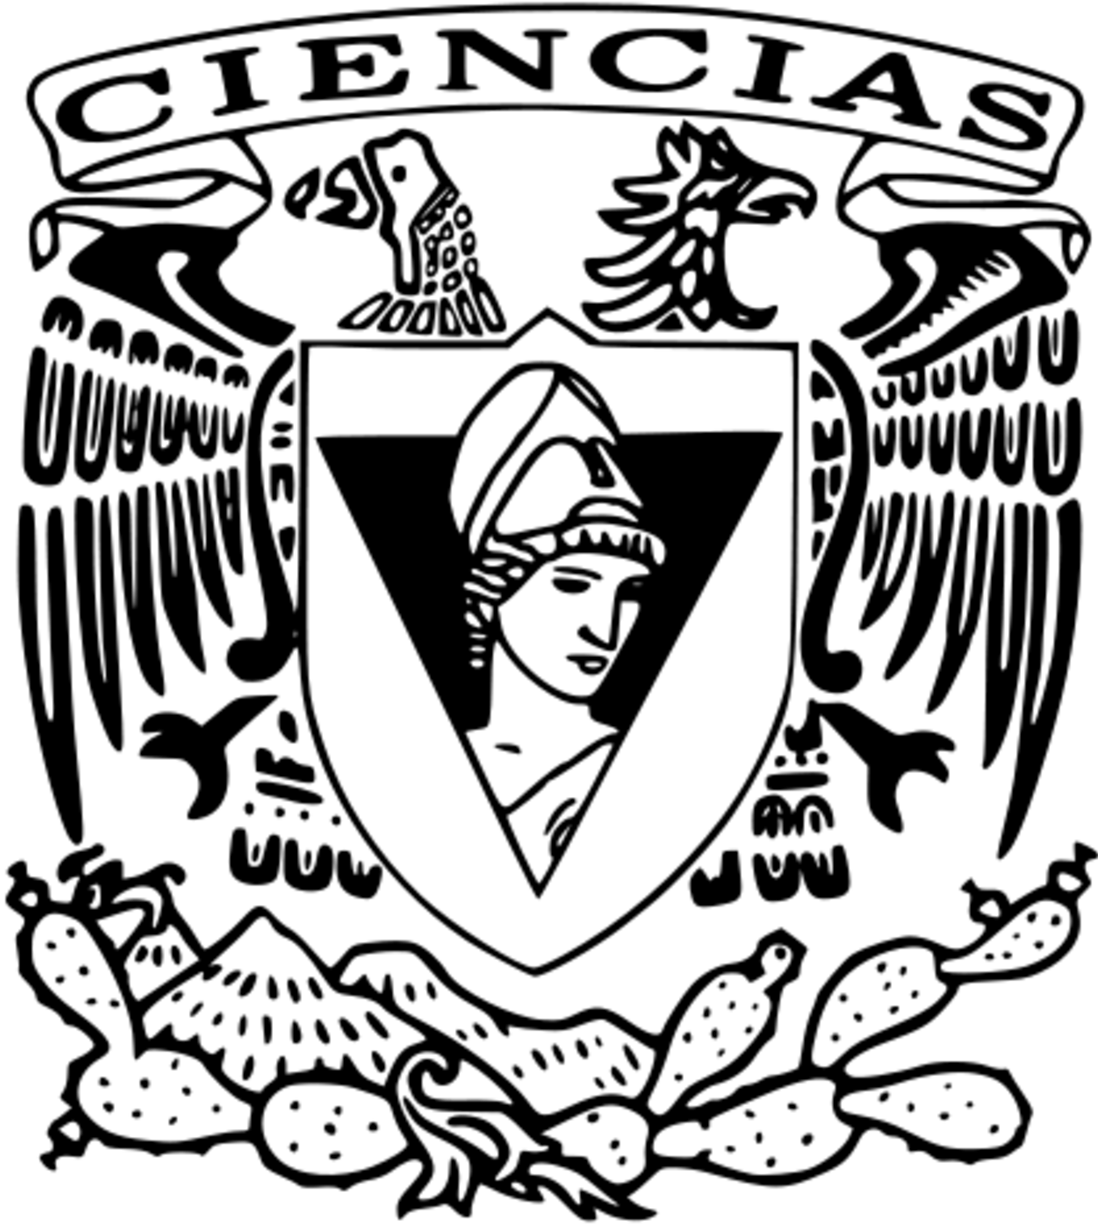
\includegraphics[height=3.4cm]{Logo_FC.png}
    	\end{center}
    \end{minipage}
\end{center}

\rule{17cm}{0.1mm}

\begin{tcolorbox}[
	title = \textcolor{black}{\textcolor{white}{Preambulo}},]
\textit{Durante mi tiempo tomando clases dentro de la facultad de ciencias de la UNAM, en la Escuela Superior de F\'isica y Matem\'aticas del IPN y
la Escuela Superior de C\'omputo del IPN he sido testigo de inumerables batallas agerridas, todas ellas centradas en un solo tema 
¿Es el $0$ un n\'umero natural?, no pude evitar formar un tab\'u en torno al tema pues no me sent\'ia lo suficientemente preparado para lograr discutir sobre este
es por ello que tome \textbf{la biblia del \'algebra superior (Laveaga)} y empece deseoso el estudio de los sistemas de Peano, para por fin hoy d\'ia
poder expresar mi postura de manera argumentada y te\'orica.
}
\end{tcolorbox}\,\\

\begin{tcolorbox}[
	title = \textcolor{black}{\textcolor{white}{Problema }},]
\textit{Sea $(N,n_0,s)$ un sistema de Peano, y sea $f:N\rightarrow N'$ una funci\'on biyectiva, definimos
$n'_0=f(n_0)\in N'$ y $s'=f\circ s \circ f^{-1}$, demuestre que $(N',n'_0,s')$ es un sistema de Peano
}
\end{tcolorbox}
\begin{proof}\,\\
    \,\\
    \textbf{i)}\,\,\,
    Es claro que $s'$ es una funci\'on inyectiva pues es composici\'on de inyectivas adem\'as afirmamos que $n'_0\notin Im (s')$, para demostrarlo
    procedemos por contradicci\'on, supongamos que $n'_0=Im(s')$, esto implica que:\,\\
    \,\\
    \begin{equation*}
        \exists\,\,\,l\in N':\,\,s'(l)=n'_0
    \end{equation*}\,\\
    Usando la definici\'on de $s'$ y $n'_0$:\,\\
    \,\\
    \begin{equation*}
        f\circ s\circ f^{-1}(l)=f(n_0)
    \end{equation*}\,\\
    Por las propiedades del sucesor $s$ se sigue que $s(f^{-1}(l))\neq n_0\in N$, y como $f$ es inyectiva\\ $f\circ s\circ f^{-1}(l)\neq f(n_0)$,
    por tanto la conclusi\'on anterior nos da una contradicci\'on, concluimos que \\$n'_0\notin Im (s')$\,\\
    \,\\
    \newpage
    \,\\
    
    \textbf{ii)}\,\,\,Pasamos al meollo del asunto definimos $T\subseteq N'$, que cumple lo siguiente:\,\\
    \begin{enumerate}
        \item $n'_0\in T$
        \item Si $r\in T$, entonces $s'(r)\in T$
    \end{enumerate}\,\\
    Sin embargo nuestra argumentaci\'on no sera en torno a este conjunto si no a un invitado
    insospechado:$f^{-1}[T]$, lo primero intersante es lo siguiente $f^{-1}[T]\subseteq N$, ahora notemos
    algo m\'as interesante aun como $n'_0\in T$ entonces $f(n_0)\in T$, por tanto
    $n_0\in f^{-1}[T]$, ahora notemos que $r\in T$ si y solo s\'i $f^{-1}(r)\in f^{-1}[T]$(esto por la biyectividad de $f$), como 
    $s'(r)\in T$ entonces $f\circ s\circ f^{-1}(r)\in T$, y por tanto $s\circ f^{-1}(r)\in f^{-1}[T]$, es decir $f^{-1}[T]$ cumple con el axioma de inducci\'on del sistema
    $(N,n_0,s)$, luego $f^{-1}[T]=N=f^{-1}[N']$, y finalmente $T=N'$ (de nuevo esto gracias a la biyectividad de $f$),  conlcuimos que en $(N',n'_0,s')$ se cumple el axioma
    de inducci\'on
\end{proof}\,\\
\,\\
Uno en primera estancia pensaria, y... ¿Esto c\'omo responde la pregunta?, este pequeño pero podersoso teorema
esconde un hecho extraordinario, si tenemos un sistema de Peano basta un solo isomorfismo entre conjuntos para construir otro, y a nivel conjuntos
como todos los sistemas de Peano son isomorfos, podriamos afirmar que estos en esencia se comportan de forma bonita
bajo cualquier biyecci\'on, en palabras llanas esto es resumido por las palabras dichas por mi profesor de \'algebra l\'ineal en ESFM:
"Puedes construir a "los naturales"  donde tu quieras, el costo es tu inducci\'on", consideremos lo siguiente:\,\\
\,\\
Sean $l:=\{1,2,3,4,5,....,n\}$ y $r:=\{0,1,2,3,4,5,6,7,8,9,...,n\}$, bajo la visi\'on extremista
alguno de estos dos conjuntos es "los naturales", el sistema de Peano, sin embargo definamos la funci\'on $f:r\rightarrow l$, tal que $f(n)=n+1$, Claramente
esta es una funci\'on biyectiva y por tanto si uno es un sistema de Peano, entonces no hay duda el otro debe serlo, es decir
$1$ es natural si y solo si $0$ es natural.\,\\
\,\\
El parrafo anterior claramente carece de la formalidad deseada a prop\'osito, nos estamos burlando de esta discusi\'on,
en esencia la pregunta si $0$ es natural o no parece bien fundamentada y debe ser respondida de inmediato, sin embargo esta pelea esconde un desconocimiento de los conceptos b\'asicos en matem\'aticas
en principio la respuesta acertada seria depende, pero ¿Por qu\'e depende?, depende a que llames tu un n\'umero natural, si un n\'umero natural
es cualquier elemento dentro de un sistema de Peano estas dando cabida a que $0$ es natural, pero no solo este es el punto polemico pues
cosas como $-1$, $-6$, o $\emptyset$ tambi\'en lo son (si no les gustaba el $0$ imagina ahora), sin embargo los n\'umeros naturales sin el $0$ tienen una raz\'on de ser
si uno define el conjunto de los n\'umeros naturales como la intersecci\'on de todos los conjuntos inductivos de $\R$ uno se dara cuenta que en efecto ni $0$ ni $-6$ ni $\emptyset$ son n\'umeros naturales.\,\\
\,\\
La conclusi\'on de todo esto es que la abstracci\'on formal de los "n\'umeros naturales" va mucho m\'as alla de estos mismos,
por tanto es natural que esta pueda abarcar una infinidad de casos donde "la esencia de los naturales existe", y  entonces ¿por qu\'e nacio toda esta pelea?, simple 
como nace cualquier pelea, un abuso de notaci\'on, es normal que en an\'alisis usemos a los naturales como la intersecci\'on de conjuntos inductivos de $\R$ para que las ideas tengan sentido, a su vez 
es obvio que en \'algebra preferimos la de sistema de Peano, sin embargo es engorroso estar mencionando cada 5 minutos que naturales son, por tanto se empezo a llamar de la misma manera a dos enfoques, dos construcciones
que est\'an encaminadas a resolver distintos problemas, derivando en lo m\'as esperado, una pelea muy divertida.



\end{document}